\documentclass[twoside]{book}

% Packages required by doxygen
\usepackage{fixltx2e}
\usepackage{calc}
\usepackage{doxygen}
\usepackage[export]{adjustbox} % also loads graphicx
\usepackage{graphicx}
\usepackage[utf8]{inputenc}
\usepackage{makeidx}
\usepackage{multicol}
\usepackage{multirow}
\PassOptionsToPackage{warn}{textcomp}
\usepackage{textcomp}
\usepackage[nointegrals]{wasysym}
\usepackage[table]{xcolor}

% Font selection
\usepackage[T1]{fontenc}
\usepackage[scaled=.90]{helvet}
\usepackage{courier}
\usepackage{amssymb}
\usepackage{sectsty}
\renewcommand{\familydefault}{\sfdefault}
\allsectionsfont{%
  \fontseries{bc}\selectfont%
  \color{darkgray}%
}
\renewcommand{\DoxyLabelFont}{%
  \fontseries{bc}\selectfont%
  \color{darkgray}%
}
\newcommand{\+}{\discretionary{\mbox{\scriptsize$\hookleftarrow$}}{}{}}

% Page & text layout
\usepackage{geometry}
\geometry{%
  a4paper,%
  top=2.5cm,%
  bottom=2.5cm,%
  left=2.5cm,%
  right=2.5cm%
}
\tolerance=750
\hfuzz=15pt
\hbadness=750
\setlength{\emergencystretch}{15pt}
\setlength{\parindent}{0cm}
\setlength{\parskip}{3ex plus 2ex minus 2ex}
\makeatletter
\renewcommand{\paragraph}{%
  \@startsection{paragraph}{4}{0ex}{-1.0ex}{1.0ex}{%
    \normalfont\normalsize\bfseries\SS@parafont%
  }%
}
\renewcommand{\subparagraph}{%
  \@startsection{subparagraph}{5}{0ex}{-1.0ex}{1.0ex}{%
    \normalfont\normalsize\bfseries\SS@subparafont%
  }%
}
\makeatother

% Headers & footers
\usepackage{fancyhdr}
\pagestyle{fancyplain}
\fancyhead[LE]{\fancyplain{}{\bfseries\thepage}}
\fancyhead[CE]{\fancyplain{}{}}
\fancyhead[RE]{\fancyplain{}{\bfseries\leftmark}}
\fancyhead[LO]{\fancyplain{}{\bfseries\rightmark}}
\fancyhead[CO]{\fancyplain{}{}}
\fancyhead[RO]{\fancyplain{}{\bfseries\thepage}}
\fancyfoot[LE]{\fancyplain{}{}}
\fancyfoot[CE]{\fancyplain{}{}}
\fancyfoot[RE]{\fancyplain{}{\bfseries\scriptsize Generated by Doxygen }}
\fancyfoot[LO]{\fancyplain{}{\bfseries\scriptsize Generated by Doxygen }}
\fancyfoot[CO]{\fancyplain{}{}}
\fancyfoot[RO]{\fancyplain{}{}}
\renewcommand{\footrulewidth}{0.4pt}
\renewcommand{\chaptermark}[1]{%
  \markboth{#1}{}%
}
\renewcommand{\sectionmark}[1]{%
  \markright{\thesection\ #1}%
}

% Indices & bibliography
\usepackage{natbib}
\usepackage[titles]{tocloft}
\setcounter{tocdepth}{3}
\setcounter{secnumdepth}{5}
\makeindex

% Hyperlinks (required, but should be loaded last)
\usepackage{ifpdf}
\ifpdf
  \usepackage[pdftex,pagebackref=true]{hyperref}
\else
  \usepackage[ps2pdf,pagebackref=true]{hyperref}
\fi
\hypersetup{%
  colorlinks=true,%
  linkcolor=blue,%
  citecolor=blue,%
  unicode%
}

% Custom commands
\newcommand{\clearemptydoublepage}{%
  \newpage{\pagestyle{empty}\cleardoublepage}%
}

\usepackage{caption}
\captionsetup{labelsep=space,justification=centering,font={bf},singlelinecheck=off,skip=4pt,position=top}

%===== C O N T E N T S =====

\begin{document}

% Titlepage & ToC
\hypersetup{pageanchor=false,
             bookmarksnumbered=true,
             pdfencoding=unicode
            }
\pagenumbering{alph}
\begin{titlepage}
\vspace*{7cm}
\begin{center}%
{\Large Embedded\+Etcher }\\
\vspace*{1cm}
{\large Generated by Doxygen 1.8.13}\\
\end{center}
\end{titlepage}
\clearemptydoublepage
\pagenumbering{roman}
\tableofcontents
\clearemptydoublepage
\pagenumbering{arabic}
\hypersetup{pageanchor=true}

%--- Begin generated contents ---
\chapter{Data Structure Index}
\section{Data Structures}
Here are the data structures with brief descriptions\+:\begin{DoxyCompactList}
\item\contentsline{section}{\hyperlink{structos_q_u_e_u_e__t}{os\+Q\+U\+E\+U\+E\+\_\+t} }{\pageref{structos_q_u_e_u_e__t}}{}
\item\contentsline{section}{\hyperlink{structos_semaphore_handle__t}{os\+Semaphore\+Handle\+\_\+t} }{\pageref{structos_semaphore_handle__t}}{}
\item\contentsline{section}{\hyperlink{structos_t_c_b__t}{os\+T\+C\+B\+\_\+t} }{\pageref{structos_t_c_b__t}}{}
\end{DoxyCompactList}

\chapter{File Index}
\section{File List}
Here is a list of all documented files with brief descriptions\+:\begin{DoxyCompactList}
\item\contentsline{section}{os/\hyperlink{error_8h}{error.\+h} \\*Error logging functionalities of the operating system }{\pageref{error_8h}}{}
\item\contentsline{section}{os/\hyperlink{heap_8h}{heap.\+h} \\*Heap implementation for the tasks of the operating system }{\pageref{heap_8h}}{}
\item\contentsline{section}{os/\hyperlink{helpers_8h}{helpers.\+h} \\*Functions, which one needs here and there for the operating system }{\pageref{helpers_8h}}{}
\item\contentsline{section}{os/\hyperlink{ossettings_8h}{ossettings.\+h} \\*File where all settings take place }{\pageref{ossettings_8h}}{}
\item\contentsline{section}{os/\hyperlink{ostypes_8h}{ostypes.\+h} \\*Different types the operating system uses are defined here }{\pageref{ostypes_8h}}{}
\item\contentsline{section}{os/\hyperlink{printf_8h}{printf.\+h} \\*Lightweight version of G\+NU printf }{\pageref{printf_8h}}{}
\item\contentsline{section}{os/\hyperlink{queues_8h}{queues.\+h} \\*Implementation for queues }{\pageref{queues_8h}}{}
\item\contentsline{section}{os/\hyperlink{scheduler_8h}{scheduler.\+h} \\*Scheduler of the operating system }{\pageref{scheduler_8h}}{}
\item\contentsline{section}{os/\hyperlink{semaphore_8h}{semaphore.\+h} \\*Mechanisms to prevent race conditions for the operating system }{\pageref{semaphore_8h}}{}
\item\contentsline{section}{platform/{\bfseries system\+\_\+timer.\+h} }{\pageref{system__timer_8h}}{}
\item\contentsline{section}{platform/{\bfseries usart.\+h} }{\pageref{usart_8h}}{}
\end{DoxyCompactList}

\chapter{Data Structure Documentation}
\hypertarget{structos_q_u_e_u_e__t}{}\section{os\+Q\+U\+E\+U\+E\+\_\+t Struct Reference}
\label{structos_q_u_e_u_e__t}\index{os\+Q\+U\+E\+U\+E\+\_\+t@{os\+Q\+U\+E\+U\+E\+\_\+t}}


{\ttfamily \#include $<$ostypes.\+h$>$}

\subsection*{Data Fields}
\begin{DoxyCompactItemize}
\item 
\mbox{\Hypertarget{structos_q_u_e_u_e__t_a418b6d1612eff43ba60ed8014917d7b1}\label{structos_q_u_e_u_e__t_a418b6d1612eff43ba60ed8014917d7b1}} 
uint8\+\_\+t {\bfseries write\+\_\+p}
\item 
\mbox{\Hypertarget{structos_q_u_e_u_e__t_a5c0e2590217d519484e519a510f4ff23}\label{structos_q_u_e_u_e__t_a5c0e2590217d519484e519a510f4ff23}} 
uint8\+\_\+t {\bfseries read\+\_\+p}
\item 
\mbox{\Hypertarget{structos_q_u_e_u_e__t_a83564fccea0d26714ccba07901241089}\label{structos_q_u_e_u_e__t_a83564fccea0d26714ccba07901241089}} 
size\+\_\+t {\bfseries varsize}
\item 
\mbox{\Hypertarget{structos_q_u_e_u_e__t_a26e55a22aa50bdfb7c20f344c19d4dd5}\label{structos_q_u_e_u_e__t_a26e55a22aa50bdfb7c20f344c19d4dd5}} 
uint16\+\_\+t {\bfseries qsize}
\item 
\mbox{\Hypertarget{structos_q_u_e_u_e__t_a53255b934b07b472175fbb8e847f9b5d}\label{structos_q_u_e_u_e__t_a53255b934b07b472175fbb8e847f9b5d}} 
void $\ast$ {\bfseries start}
\end{DoxyCompactItemize}


\subsection{Detailed Description}
Data type holds a void pointer to an array to be able to use the queues for many data types. 

The documentation for this struct was generated from the following file\+:\begin{DoxyCompactItemize}
\item 
os/\hyperlink{ostypes_8h}{ostypes.\+h}\end{DoxyCompactItemize}

\hypertarget{structos_semaphore_handle__t}{}\section{os\+Semaphore\+Handle\+\_\+t Struct Reference}
\label{structos_semaphore_handle__t}\index{os\+Semaphore\+Handle\+\_\+t@{os\+Semaphore\+Handle\+\_\+t}}
\subsection*{Data Fields}
\begin{DoxyCompactItemize}
\item 
\mbox{\Hypertarget{structos_semaphore_handle__t_a5a84f06656d71ab4080d24ca01c6507f}\label{structos_semaphore_handle__t_a5a84f06656d71ab4080d24ca01c6507f}} 
os\+Semaphore\+Type\+\_\+t {\bfseries type}
\item 
\mbox{\Hypertarget{structos_semaphore_handle__t_a325819a8e492ac69542e8b31705af6e9}\label{structos_semaphore_handle__t_a325819a8e492ac69542e8b31705af6e9}} 
uint8\+\_\+t {\bfseries data}
\end{DoxyCompactItemize}


The documentation for this struct was generated from the following file\+:\begin{DoxyCompactItemize}
\item 
os/\hyperlink{ostypes_8h}{ostypes.\+h}\end{DoxyCompactItemize}

\hypertarget{structos_t_c_b__t}{}\section{os\+T\+C\+B\+\_\+t Struct Reference}
\label{structos_t_c_b__t}\index{os\+T\+C\+B\+\_\+t@{os\+T\+C\+B\+\_\+t}}


{\ttfamily \#include $<$ostypes.\+h$>$}

\subsection*{Data Fields}
\begin{DoxyCompactItemize}
\item 
\mbox{\Hypertarget{structos_t_c_b__t_aa99c587c00df01f56baf5c6e46c46361}\label{structos_t_c_b__t_aa99c587c00df01f56baf5c6e46c46361}} 
void($\ast$ {\bfseries fnc\+\_\+ptr} )(void $\ast$)
\item 
\mbox{\Hypertarget{structos_t_c_b__t_a053fb83c9604d11fa3b97113a1cee7c9}\label{structos_t_c_b__t_a053fb83c9604d11fa3b97113a1cee7c9}} 
char {\bfseries name} \mbox{[}M\+A\+X\+\_\+\+S\+I\+Z\+E\+\_\+\+T\+A\+S\+K\+\_\+\+N\+A\+ME\mbox{]}
\item 
\mbox{\Hypertarget{structos_t_c_b__t_ab019aab8795fa409075f1956083bfd62}\label{structos_t_c_b__t_ab019aab8795fa409075f1956083bfd62}} 
void $\ast$ {\bfseries arguments}
\item 
\mbox{\Hypertarget{structos_t_c_b__t_a0ad043071ccc7a261d79a759dc9c6f0c}\label{structos_t_c_b__t_a0ad043071ccc7a261d79a759dc9c6f0c}} 
uint8\+\_\+t {\bfseries priority}
\item 
\mbox{\Hypertarget{structos_t_c_b__t_a602c451f173294fef0097bb86d082602}\label{structos_t_c_b__t_a602c451f173294fef0097bb86d082602}} 
\hyperlink{ostypes_8h_ae410cf8fbf1704d3cedf2e2648b94a55}{os\+Task\+State\+\_\+t} {\bfseries state}
\item 
\mbox{\Hypertarget{structos_t_c_b__t_aabdd8be14846d97f622cacdbdaaa5925}\label{structos_t_c_b__t_aabdd8be14846d97f622cacdbdaaa5925}} 
uint32\+\_\+t {\bfseries wake\+\_\+up}
\end{DoxyCompactItemize}


\subsection{Detailed Description}
Struct representing the task control block. 

The documentation for this struct was generated from the following file\+:\begin{DoxyCompactItemize}
\item 
os/\hyperlink{ostypes_8h}{ostypes.\+h}\end{DoxyCompactItemize}

\chapter{File Documentation}
\hypertarget{error_8h}{}\section{os/error.h File Reference}
\label{error_8h}\index{os/error.\+h@{os/error.\+h}}


Error logging functionalities of the operating system.  


{\ttfamily \#include \char`\"{}ostypes.\+h\char`\"{}}\newline
{\ttfamily \#include \char`\"{}ossettings.\+h\char`\"{}}\newline
Include dependency graph for error.\+h\+:
\nopagebreak
\begin{figure}[H]
\begin{center}
\leavevmode
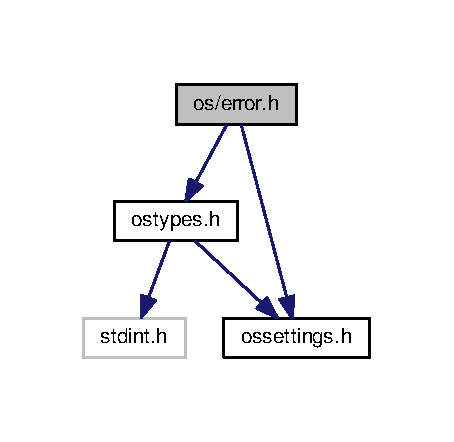
\includegraphics[width=218pt]{error_8h__incl}
\end{center}
\end{figure}
\subsection*{Macros}
\begin{DoxyCompactItemize}
\item 
\#define \hyperlink{error_8h_ad43da790cc069011db9c6f0ef8fea11b}{D\+E\+B\+U\+G\+\_\+\+M\+SG}(M\+SG, ...)
\item 
\#define \hyperlink{error_8h_a443fea42d93b53e3569d33e80c5de6c4}{T\+H\+R\+O\+W\+\_\+\+E\+R\+R\+OR}(E\+R\+R\+O\+R\+\_\+\+T\+Y\+PE)~\hyperlink{error_8h_a540c46d0a32421cad29354147a02c4ea}{os\+Print\+Error}(\+\_\+\+\_\+\+F\+I\+L\+E\+\_\+\+\_\+, \+\_\+\+\_\+\+L\+I\+N\+E\+\_\+\+\_\+, E\+R\+R\+O\+R\+\_\+\+T\+Y\+PE)
\item 
\#define \hyperlink{error_8h_a22fc1f25f5e596198d4a773df7762c77}{T\+H\+R\+O\+W\+\_\+\+W\+A\+R\+N\+I\+NG}(W\+A\+R\+N\+I\+N\+G\+\_\+\+T\+Y\+PE)~\hyperlink{error_8h_a8ea68ece7fa351c9c046006749706e26}{os\+Print\+Warning}(\+\_\+\+\_\+\+F\+I\+L\+E\+\_\+\+\_\+, \+\_\+\+\_\+\+L\+I\+N\+E\+\_\+\+\_\+, W\+A\+R\+N\+I\+N\+G\+\_\+\+T\+Y\+PE)
\end{DoxyCompactItemize}
\subsection*{Functions}
\begin{DoxyCompactItemize}
\item 
uint8\+\_\+t \hyperlink{error_8h_af770cfb23cba6e7aa7c69aad1bbf968c}{os\+Explain\+Error} (const char $\ast$ifile, const uint8\+\_\+t iline, const \hyperlink{ostypes_8h_acd9f76a1fbd8bc9084ff34add637094f}{os\+Error\+\_\+t} ierror, char $\ast$iomessage)
\item 
uint8\+\_\+t \hyperlink{error_8h_a540c46d0a32421cad29354147a02c4ea}{os\+Print\+Error} (const char $\ast$ifile, const int iline, const \hyperlink{ostypes_8h_acd9f76a1fbd8bc9084ff34add637094f}{os\+Error\+\_\+t} ierror)
\item 
uint8\+\_\+t \hyperlink{error_8h_a29238a23e284dd0a6278434447be4682}{os\+Explain\+Warning} (const char $\ast$ifile, const uint8\+\_\+t iline, const \hyperlink{ostypes_8h_a5c976ef3f21f800d03382e5cc640c362}{os\+Warning\+\_\+t} ierror, char $\ast$iomessage)
\item 
uint8\+\_\+t \hyperlink{error_8h_a8ea68ece7fa351c9c046006749706e26}{os\+Print\+Warning} (const char $\ast$ifile, const int iline, const \hyperlink{ostypes_8h_a5c976ef3f21f800d03382e5cc640c362}{os\+Warning\+\_\+t} ierror)
\end{DoxyCompactItemize}


\subsection{Detailed Description}
Error logging functionalities of the operating system. 

\begin{DoxyAuthor}{Author}
Maximilian Stiefel 
\end{DoxyAuthor}
\begin{DoxyDate}{Date}
8 Jan 2018 
\end{DoxyDate}


\subsection{Macro Definition Documentation}
\mbox{\Hypertarget{error_8h_ad43da790cc069011db9c6f0ef8fea11b}\label{error_8h_ad43da790cc069011db9c6f0ef8fea11b}} 
\index{error.\+h@{error.\+h}!D\+E\+B\+U\+G\+\_\+\+M\+SG@{D\+E\+B\+U\+G\+\_\+\+M\+SG}}
\index{D\+E\+B\+U\+G\+\_\+\+M\+SG@{D\+E\+B\+U\+G\+\_\+\+M\+SG}!error.\+h@{error.\+h}}
\subsubsection{\texorpdfstring{D\+E\+B\+U\+G\+\_\+\+M\+SG}{DEBUG\_MSG}}
{\footnotesize\ttfamily \#define D\+E\+B\+U\+G\+\_\+\+M\+SG(\begin{DoxyParamCaption}\item[{}]{M\+SG,  }\item[{}]{... }\end{DoxyParamCaption})}

Create smart debug messages, which are disable if D\+E\+B\+UG is not defined. \mbox{\Hypertarget{error_8h_a443fea42d93b53e3569d33e80c5de6c4}\label{error_8h_a443fea42d93b53e3569d33e80c5de6c4}} 
\index{error.\+h@{error.\+h}!T\+H\+R\+O\+W\+\_\+\+E\+R\+R\+OR@{T\+H\+R\+O\+W\+\_\+\+E\+R\+R\+OR}}
\index{T\+H\+R\+O\+W\+\_\+\+E\+R\+R\+OR@{T\+H\+R\+O\+W\+\_\+\+E\+R\+R\+OR}!error.\+h@{error.\+h}}
\subsubsection{\texorpdfstring{T\+H\+R\+O\+W\+\_\+\+E\+R\+R\+OR}{THROW\_ERROR}}
{\footnotesize\ttfamily \#define T\+H\+R\+O\+W\+\_\+\+E\+R\+R\+OR(\begin{DoxyParamCaption}\item[{}]{E\+R\+R\+O\+R\+\_\+\+T\+Y\+PE }\end{DoxyParamCaption})~\hyperlink{error_8h_a540c46d0a32421cad29354147a02c4ea}{os\+Print\+Error}(\+\_\+\+\_\+\+F\+I\+L\+E\+\_\+\+\_\+, \+\_\+\+\_\+\+L\+I\+N\+E\+\_\+\+\_\+, E\+R\+R\+O\+R\+\_\+\+T\+Y\+PE)}

Throws an error given an error type. \mbox{\Hypertarget{error_8h_a22fc1f25f5e596198d4a773df7762c77}\label{error_8h_a22fc1f25f5e596198d4a773df7762c77}} 
\index{error.\+h@{error.\+h}!T\+H\+R\+O\+W\+\_\+\+W\+A\+R\+N\+I\+NG@{T\+H\+R\+O\+W\+\_\+\+W\+A\+R\+N\+I\+NG}}
\index{T\+H\+R\+O\+W\+\_\+\+W\+A\+R\+N\+I\+NG@{T\+H\+R\+O\+W\+\_\+\+W\+A\+R\+N\+I\+NG}!error.\+h@{error.\+h}}
\subsubsection{\texorpdfstring{T\+H\+R\+O\+W\+\_\+\+W\+A\+R\+N\+I\+NG}{THROW\_WARNING}}
{\footnotesize\ttfamily \#define T\+H\+R\+O\+W\+\_\+\+W\+A\+R\+N\+I\+NG(\begin{DoxyParamCaption}\item[{}]{W\+A\+R\+N\+I\+N\+G\+\_\+\+T\+Y\+PE }\end{DoxyParamCaption})~\hyperlink{error_8h_a8ea68ece7fa351c9c046006749706e26}{os\+Print\+Warning}(\+\_\+\+\_\+\+F\+I\+L\+E\+\_\+\+\_\+, \+\_\+\+\_\+\+L\+I\+N\+E\+\_\+\+\_\+, W\+A\+R\+N\+I\+N\+G\+\_\+\+T\+Y\+PE)}

Throws a warning given a warning type. 

\subsection{Function Documentation}
\mbox{\Hypertarget{error_8h_af770cfb23cba6e7aa7c69aad1bbf968c}\label{error_8h_af770cfb23cba6e7aa7c69aad1bbf968c}} 
\index{error.\+h@{error.\+h}!os\+Explain\+Error@{os\+Explain\+Error}}
\index{os\+Explain\+Error@{os\+Explain\+Error}!error.\+h@{error.\+h}}
\subsubsection{\texorpdfstring{os\+Explain\+Error()}{osExplainError()}}
{\footnotesize\ttfamily uint8\+\_\+t os\+Explain\+Error (\begin{DoxyParamCaption}\item[{const char $\ast$}]{ifile,  }\item[{const uint8\+\_\+t}]{iline,  }\item[{const \hyperlink{ostypes_8h_acd9f76a1fbd8bc9084ff34add637094f}{os\+Error\+\_\+t}}]{ierror,  }\item[{char $\ast$}]{iomessage }\end{DoxyParamCaption})}

Creating a error message string from inter alia an error code.


\begin{DoxyParams}{Parameters}
{\em ifile} & Filename where error occurs. \\
\hline
{\em iline} & Line where error occurs. \\
\hline
{\em ierror} & Error code. \\
\hline
{\em message} & Message related to the error. \\
\hline
\end{DoxyParams}

\begin{DoxyRetVals}{Return values}
{\em 1} & (S\+U\+C\+C\+E\+SS) or 0 (F\+A\+I\+L\+U\+RE). \\
\hline
\end{DoxyRetVals}
\mbox{\Hypertarget{error_8h_a29238a23e284dd0a6278434447be4682}\label{error_8h_a29238a23e284dd0a6278434447be4682}} 
\index{error.\+h@{error.\+h}!os\+Explain\+Warning@{os\+Explain\+Warning}}
\index{os\+Explain\+Warning@{os\+Explain\+Warning}!error.\+h@{error.\+h}}
\subsubsection{\texorpdfstring{os\+Explain\+Warning()}{osExplainWarning()}}
{\footnotesize\ttfamily uint8\+\_\+t os\+Explain\+Warning (\begin{DoxyParamCaption}\item[{const char $\ast$}]{ifile,  }\item[{const uint8\+\_\+t}]{iline,  }\item[{const \hyperlink{ostypes_8h_a5c976ef3f21f800d03382e5cc640c362}{os\+Warning\+\_\+t}}]{ierror,  }\item[{char $\ast$}]{iomessage }\end{DoxyParamCaption})}

Creating a warning message string from inter alia a warning code.


\begin{DoxyParams}{Parameters}
{\em ifile} & Filename where warning occurs. \\
\hline
{\em iline} & Line where warning occurs. \\
\hline
{\em ierror} & Warning code. \\
\hline
{\em message} & Message related to the warning. \\
\hline
\end{DoxyParams}

\begin{DoxyRetVals}{Return values}
{\em 1} & (S\+U\+C\+C\+E\+SS) or 0 (F\+A\+I\+L\+U\+RE). \\
\hline
\end{DoxyRetVals}
\mbox{\Hypertarget{error_8h_a540c46d0a32421cad29354147a02c4ea}\label{error_8h_a540c46d0a32421cad29354147a02c4ea}} 
\index{error.\+h@{error.\+h}!os\+Print\+Error@{os\+Print\+Error}}
\index{os\+Print\+Error@{os\+Print\+Error}!error.\+h@{error.\+h}}
\subsubsection{\texorpdfstring{os\+Print\+Error()}{osPrintError()}}
{\footnotesize\ttfamily uint8\+\_\+t os\+Print\+Error (\begin{DoxyParamCaption}\item[{const char $\ast$}]{ifile,  }\item[{const int}]{iline,  }\item[{const \hyperlink{ostypes_8h_acd9f76a1fbd8bc9084ff34add637094f}{os\+Error\+\_\+t}}]{ierror }\end{DoxyParamCaption})}

Print error. This is where the error output can be redirected (later).


\begin{DoxyParams}{Parameters}
{\em ifile} & Filename where error occurs. \\
\hline
{\em iline} & Line where error occurs. \\
\hline
{\em ierror} & Error code. \\
\hline
\end{DoxyParams}

\begin{DoxyRetVals}{Return values}
{\em 1} & (S\+U\+C\+C\+E\+SS) or 0 (F\+A\+I\+L\+U\+RE). \\
\hline
\end{DoxyRetVals}
\mbox{\Hypertarget{error_8h_a8ea68ece7fa351c9c046006749706e26}\label{error_8h_a8ea68ece7fa351c9c046006749706e26}} 
\index{error.\+h@{error.\+h}!os\+Print\+Warning@{os\+Print\+Warning}}
\index{os\+Print\+Warning@{os\+Print\+Warning}!error.\+h@{error.\+h}}
\subsubsection{\texorpdfstring{os\+Print\+Warning()}{osPrintWarning()}}
{\footnotesize\ttfamily uint8\+\_\+t os\+Print\+Warning (\begin{DoxyParamCaption}\item[{const char $\ast$}]{ifile,  }\item[{const int}]{iline,  }\item[{const \hyperlink{ostypes_8h_a5c976ef3f21f800d03382e5cc640c362}{os\+Warning\+\_\+t}}]{ierror }\end{DoxyParamCaption})}

Print warning. This is where the warning output can be redirected (later).


\begin{DoxyParams}{Parameters}
{\em ifile} & Filename where warning occurs. \\
\hline
{\em iline} & Line where warning occurs. \\
\hline
{\em ierror} & Warning code. \\
\hline
\end{DoxyParams}

\begin{DoxyRetVals}{Return values}
{\em 1} & (S\+U\+C\+C\+E\+SS) or 0 (F\+A\+I\+L\+U\+RE). \\
\hline
\end{DoxyRetVals}

\hypertarget{heap_8h}{}\section{os/heap.h File Reference}
\label{heap_8h}\index{os/heap.\+h@{os/heap.\+h}}


Heap implementation for the tasks of the operating system.  


{\ttfamily \#include \char`\"{}ostypes.\+h\char`\"{}}\newline
Include dependency graph for heap.\+h\+:
\nopagebreak
\begin{figure}[H]
\begin{center}
\leavevmode
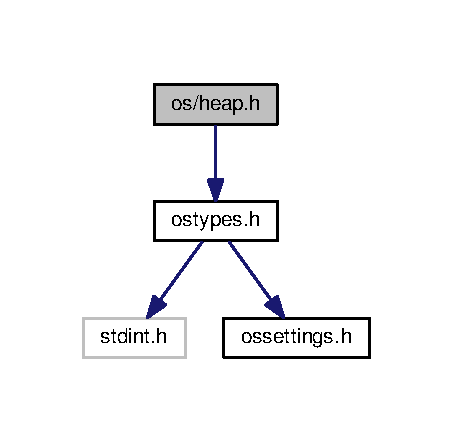
\includegraphics[width=218pt]{heap_8h__incl}
\end{center}
\end{figure}
\subsection*{Functions}
\begin{DoxyCompactItemize}
\item 
void \hyperlink{heap_8h_ae4c24d26f4411ab5492a2cc8dd5a4e7c}{os\+Heap\+Init} (\hyperlink{ostypes_8h_a7b59ec4a57312624d7d832ba4a8e04be}{os\+Heap\+Node\+\_\+t} $\ast$ioarray)
\item 
void \hyperlink{heap_8h_a5a51c0aca53767d5038681cc649d5fa8}{os\+Heap\+Heapify} (\hyperlink{ostypes_8h_a7b59ec4a57312624d7d832ba4a8e04be}{os\+Heap\+Node\+\_\+t} $\ast$ioarray, uint8\+\_\+t iind)
\item 
void \hyperlink{heap_8h_aba6f21f0421450da6531c7ea9f6976b5}{os\+Heap\+Build} (\hyperlink{ostypes_8h_a7b59ec4a57312624d7d832ba4a8e04be}{os\+Heap\+Node\+\_\+t} $\ast$ioarray)
\item 
uint8\+\_\+t \hyperlink{heap_8h_a2a73414cf2e4e1d2cebb4597a36bc018}{os\+Heap\+Maximum} (\hyperlink{ostypes_8h_a7b59ec4a57312624d7d832ba4a8e04be}{os\+Heap\+Node\+\_\+t} $\ast$ioarray, \hyperlink{ostypes_8h_a7b59ec4a57312624d7d832ba4a8e04be}{os\+Heap\+Node\+\_\+t} $\ast$iomax)
\item 
uint8\+\_\+t \hyperlink{heap_8h_a31002fadb05f80382c9714462dfb092e}{os\+Heap\+Extract\+Maximum} (\hyperlink{ostypes_8h_a7b59ec4a57312624d7d832ba4a8e04be}{os\+Heap\+Node\+\_\+t} $\ast$ioarray, \hyperlink{ostypes_8h_a7b59ec4a57312624d7d832ba4a8e04be}{os\+Heap\+Node\+\_\+t} $\ast$iomax)
\item 
uint8\+\_\+t \hyperlink{heap_8h_ab5c1d9c908e7d618bd5869f6e0ed16c5}{os\+Heap\+Insert} (\hyperlink{ostypes_8h_a7b59ec4a57312624d7d832ba4a8e04be}{os\+Heap\+Node\+\_\+t} $\ast$ioarray, \hyperlink{ostypes_8h_a7b59ec4a57312624d7d832ba4a8e04be}{os\+Heap\+Node\+\_\+t} x)
\item 
void \hyperlink{heap_8h_abfcd76f5650f218825578b0bd1652587}{os\+Heap\+PrintS} (\hyperlink{ostypes_8h_a7b59ec4a57312624d7d832ba4a8e04be}{os\+Heap\+Node\+\_\+t} $\ast$ioarray)
\item 
uint8\+\_\+t \hyperlink{heap_8h_a999a4beae27d4c7085278724feeabbc1}{os\+Heap\+Is\+Empty} (\hyperlink{ostypes_8h_a7b59ec4a57312624d7d832ba4a8e04be}{os\+Heap\+Node\+\_\+t} $\ast$ioarray)
\end{DoxyCompactItemize}


\subsection{Detailed Description}
Heap implementation for the tasks of the operating system. 

\begin{DoxyAuthor}{Author}
Maximilian Stiefel 
\end{DoxyAuthor}
\begin{DoxyDate}{Date}
8 Jan 2018 
\end{DoxyDate}


\subsection{Function Documentation}
\mbox{\Hypertarget{heap_8h_aba6f21f0421450da6531c7ea9f6976b5}\label{heap_8h_aba6f21f0421450da6531c7ea9f6976b5}} 
\index{heap.\+h@{heap.\+h}!os\+Heap\+Build@{os\+Heap\+Build}}
\index{os\+Heap\+Build@{os\+Heap\+Build}!heap.\+h@{heap.\+h}}
\subsubsection{\texorpdfstring{os\+Heap\+Build()}{osHeapBuild()}}
{\footnotesize\ttfamily void os\+Heap\+Build (\begin{DoxyParamCaption}\item[{\hyperlink{ostypes_8h_a7b59ec4a57312624d7d832ba4a8e04be}{os\+Heap\+Node\+\_\+t} $\ast$}]{ioarray }\end{DoxyParamCaption})}

Build the heap from the bottom up. Given an array which is not heapified at all.


\begin{DoxyParams}{Parameters}
{\em ioarray} & Array where the heap is stored. \\
\hline
\end{DoxyParams}
\mbox{\Hypertarget{heap_8h_a31002fadb05f80382c9714462dfb092e}\label{heap_8h_a31002fadb05f80382c9714462dfb092e}} 
\index{heap.\+h@{heap.\+h}!os\+Heap\+Extract\+Maximum@{os\+Heap\+Extract\+Maximum}}
\index{os\+Heap\+Extract\+Maximum@{os\+Heap\+Extract\+Maximum}!heap.\+h@{heap.\+h}}
\subsubsection{\texorpdfstring{os\+Heap\+Extract\+Maximum()}{osHeapExtractMaximum()}}
{\footnotesize\ttfamily uint8\+\_\+t os\+Heap\+Extract\+Maximum (\begin{DoxyParamCaption}\item[{\hyperlink{ostypes_8h_a7b59ec4a57312624d7d832ba4a8e04be}{os\+Heap\+Node\+\_\+t} $\ast$}]{ioarray,  }\item[{\hyperlink{ostypes_8h_a7b59ec4a57312624d7d832ba4a8e04be}{os\+Heap\+Node\+\_\+t} $\ast$}]{iomax }\end{DoxyParamCaption})}

Copy heap maximum and remove it (extract).


\begin{DoxyParams}{Parameters}
{\em ioarray} & Array where the heap is stored. \\
\hline
{\em iomax} & Node, which is the maximum. \\
\hline
\end{DoxyParams}

\begin{DoxyRetVals}{Return values}
{\em 1} & (S\+U\+C\+C\+E\+SS) or 0 (heap is empty). \\
\hline
\end{DoxyRetVals}
\mbox{\Hypertarget{heap_8h_a5a51c0aca53767d5038681cc649d5fa8}\label{heap_8h_a5a51c0aca53767d5038681cc649d5fa8}} 
\index{heap.\+h@{heap.\+h}!os\+Heap\+Heapify@{os\+Heap\+Heapify}}
\index{os\+Heap\+Heapify@{os\+Heap\+Heapify}!heap.\+h@{heap.\+h}}
\subsubsection{\texorpdfstring{os\+Heap\+Heapify()}{osHeapHeapify()}}
{\footnotesize\ttfamily void os\+Heap\+Heapify (\begin{DoxyParamCaption}\item[{\hyperlink{ostypes_8h_a7b59ec4a57312624d7d832ba4a8e04be}{os\+Heap\+Node\+\_\+t} $\ast$}]{ioarray,  }\item[{uint8\+\_\+t}]{iind }\end{DoxyParamCaption})}

Classic heapify operation.


\begin{DoxyParams}{Parameters}
{\em ioarray} & Array where the heap is stored. \\
\hline
{\em iind} & Element to be put in the right place. \\
\hline
\end{DoxyParams}
\mbox{\Hypertarget{heap_8h_ae4c24d26f4411ab5492a2cc8dd5a4e7c}\label{heap_8h_ae4c24d26f4411ab5492a2cc8dd5a4e7c}} 
\index{heap.\+h@{heap.\+h}!os\+Heap\+Init@{os\+Heap\+Init}}
\index{os\+Heap\+Init@{os\+Heap\+Init}!heap.\+h@{heap.\+h}}
\subsubsection{\texorpdfstring{os\+Heap\+Init()}{osHeapInit()}}
{\footnotesize\ttfamily void os\+Heap\+Init (\begin{DoxyParamCaption}\item[{\hyperlink{ostypes_8h_a7b59ec4a57312624d7d832ba4a8e04be}{os\+Heap\+Node\+\_\+t} $\ast$}]{ioarray }\end{DoxyParamCaption})}

Initializes all heap elements by setting them to N\+U\+LL.


\begin{DoxyParams}{Parameters}
{\em Array} & where the heap is stored. \\
\hline
\end{DoxyParams}
\mbox{\Hypertarget{heap_8h_ab5c1d9c908e7d618bd5869f6e0ed16c5}\label{heap_8h_ab5c1d9c908e7d618bd5869f6e0ed16c5}} 
\index{heap.\+h@{heap.\+h}!os\+Heap\+Insert@{os\+Heap\+Insert}}
\index{os\+Heap\+Insert@{os\+Heap\+Insert}!heap.\+h@{heap.\+h}}
\subsubsection{\texorpdfstring{os\+Heap\+Insert()}{osHeapInsert()}}
{\footnotesize\ttfamily uint8\+\_\+t os\+Heap\+Insert (\begin{DoxyParamCaption}\item[{\hyperlink{ostypes_8h_a7b59ec4a57312624d7d832ba4a8e04be}{os\+Heap\+Node\+\_\+t} $\ast$}]{ioarray,  }\item[{\hyperlink{ostypes_8h_a7b59ec4a57312624d7d832ba4a8e04be}{os\+Heap\+Node\+\_\+t}}]{x }\end{DoxyParamCaption})}

Insert a node into the heap.


\begin{DoxyParams}{Parameters}
{\em ioarray} & Array where the heap is stored. \\
\hline
{\em x} & Node to be inserted into the heap. \\
\hline
\end{DoxyParams}

\begin{DoxyRetVals}{Return values}
{\em 1} & (S\+U\+C\+C\+E\+SS) or 0 (heap is full). \\
\hline
\end{DoxyRetVals}
\mbox{\Hypertarget{heap_8h_a999a4beae27d4c7085278724feeabbc1}\label{heap_8h_a999a4beae27d4c7085278724feeabbc1}} 
\index{heap.\+h@{heap.\+h}!os\+Heap\+Is\+Empty@{os\+Heap\+Is\+Empty}}
\index{os\+Heap\+Is\+Empty@{os\+Heap\+Is\+Empty}!heap.\+h@{heap.\+h}}
\subsubsection{\texorpdfstring{os\+Heap\+Is\+Empty()}{osHeapIsEmpty()}}
{\footnotesize\ttfamily uint8\+\_\+t os\+Heap\+Is\+Empty (\begin{DoxyParamCaption}\item[{\hyperlink{ostypes_8h_a7b59ec4a57312624d7d832ba4a8e04be}{os\+Heap\+Node\+\_\+t} $\ast$}]{ioarray }\end{DoxyParamCaption})}

Is the heap empty?


\begin{DoxyParams}{Parameters}
{\em ioarray} & Array where the heap is stored. \\
\hline
\end{DoxyParams}
\mbox{\Hypertarget{heap_8h_a2a73414cf2e4e1d2cebb4597a36bc018}\label{heap_8h_a2a73414cf2e4e1d2cebb4597a36bc018}} 
\index{heap.\+h@{heap.\+h}!os\+Heap\+Maximum@{os\+Heap\+Maximum}}
\index{os\+Heap\+Maximum@{os\+Heap\+Maximum}!heap.\+h@{heap.\+h}}
\subsubsection{\texorpdfstring{os\+Heap\+Maximum()}{osHeapMaximum()}}
{\footnotesize\ttfamily uint8\+\_\+t os\+Heap\+Maximum (\begin{DoxyParamCaption}\item[{\hyperlink{ostypes_8h_a7b59ec4a57312624d7d832ba4a8e04be}{os\+Heap\+Node\+\_\+t} $\ast$}]{ioarray,  }\item[{\hyperlink{ostypes_8h_a7b59ec4a57312624d7d832ba4a8e04be}{os\+Heap\+Node\+\_\+t} $\ast$}]{iomax }\end{DoxyParamCaption})}

Copy heap maximum.


\begin{DoxyParams}{Parameters}
{\em ioarray} & Array where the heap is stored. \\
\hline
{\em iomax} & Node, which is the maximum. \\
\hline
\end{DoxyParams}

\begin{DoxyRetVals}{Return values}
{\em 1} & (S\+U\+C\+C\+E\+SS) or 0 (heap is empty). \\
\hline
\end{DoxyRetVals}
\mbox{\Hypertarget{heap_8h_abfcd76f5650f218825578b0bd1652587}\label{heap_8h_abfcd76f5650f218825578b0bd1652587}} 
\index{heap.\+h@{heap.\+h}!os\+Heap\+PrintS@{os\+Heap\+PrintS}}
\index{os\+Heap\+PrintS@{os\+Heap\+PrintS}!heap.\+h@{heap.\+h}}
\subsubsection{\texorpdfstring{os\+Heap\+Print\+S()}{osHeapPrintS()}}
{\footnotesize\ttfamily void os\+Heap\+PrintS (\begin{DoxyParamCaption}\item[{\hyperlink{ostypes_8h_a7b59ec4a57312624d7d832ba4a8e04be}{os\+Heap\+Node\+\_\+t} $\ast$}]{ioarray }\end{DoxyParamCaption})}

Print heap all priorities for debugging purposes.


\begin{DoxyParams}{Parameters}
{\em ioarray} & Array where the heap is stored. \\
\hline
\end{DoxyParams}

\hypertarget{helpers_8h}{}\section{os/helpers.h File Reference}
\label{helpers_8h}\index{os/helpers.\+h@{os/helpers.\+h}}


Functions, which one needs here and there for the operating system.  


{\ttfamily \#include \char`\"{}stm32f10x.\+h\char`\"{}}\newline
{\ttfamily \#include $<$stdlib.\+h$>$}\newline
Include dependency graph for helpers.\+h\+:\nopagebreak
\begin{figure}[H]
\begin{center}
\leavevmode
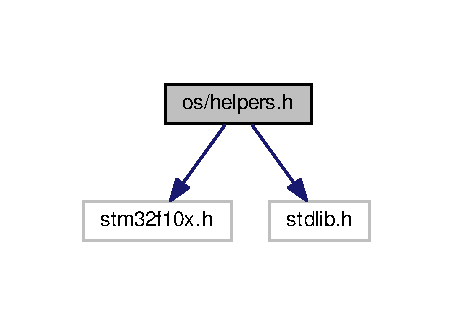
\includegraphics[width=218pt]{helpers_8h__incl}
\end{center}
\end{figure}
\subsection*{Functions}
\begin{DoxyCompactItemize}
\item 
int \hyperlink{helpers_8h_a8f7c8ca9321d4fa5a07c09b42120cab9}{os\+Pow\+Int} (int ibase, int iexponent)
\item 
uint8\+\_\+t \hyperlink{helpers_8h_a47defb2893c0a5e4427dd9daf6d5057d}{os\+Itoa} (int iint, char $\ast$iochar, size\+\_\+t ibuffsize, size\+\_\+t $\ast$obuffsize)
\end{DoxyCompactItemize}


\subsection{Detailed Description}
Functions, which one needs here and there for the operating system. 

\begin{DoxyAuthor}{Author}
Maximilian Stiefel 
\end{DoxyAuthor}
\begin{DoxyDate}{Date}
8 Jan 2018 
\end{DoxyDate}


\subsection{Function Documentation}
\mbox{\Hypertarget{helpers_8h_a47defb2893c0a5e4427dd9daf6d5057d}\label{helpers_8h_a47defb2893c0a5e4427dd9daf6d5057d}} 
\index{helpers.\+h@{helpers.\+h}!os\+Itoa@{os\+Itoa}}
\index{os\+Itoa@{os\+Itoa}!helpers.\+h@{helpers.\+h}}
\subsubsection{\texorpdfstring{os\+Itoa()}{osItoa()}}
{\footnotesize\ttfamily uint8\+\_\+t os\+Itoa (\begin{DoxyParamCaption}\item[{int}]{iint,  }\item[{char $\ast$}]{iochar,  }\item[{size\+\_\+t}]{ibuffsize,  }\item[{size\+\_\+t $\ast$}]{obuffsize }\end{DoxyParamCaption})}

Simple Interger to A\+S\+C\+II conversion.


\begin{DoxyParams}{Parameters}
{\em iint} & Input integer. \\
\hline
{\em iochar} & C string where the result ends up. \\
\hline
{\em ibuffsize} & Size of the C string for security reasons. \\
\hline
{\em obuffsize} & Size of the string created by the function. \\
\hline
\end{DoxyParams}

\begin{DoxyRetVals}{Return values}
{\em 1} & (S\+U\+C\+C\+E\+SS) or 0 (buffer overflow). \\
\hline
\end{DoxyRetVals}
\mbox{\Hypertarget{helpers_8h_a8f7c8ca9321d4fa5a07c09b42120cab9}\label{helpers_8h_a8f7c8ca9321d4fa5a07c09b42120cab9}} 
\index{helpers.\+h@{helpers.\+h}!os\+Pow\+Int@{os\+Pow\+Int}}
\index{os\+Pow\+Int@{os\+Pow\+Int}!helpers.\+h@{helpers.\+h}}
\subsubsection{\texorpdfstring{os\+Pow\+Int()}{osPowInt()}}
{\footnotesize\ttfamily int os\+Pow\+Int (\begin{DoxyParamCaption}\item[{int}]{ibase,  }\item[{int}]{iexponent }\end{DoxyParamCaption})\hspace{0.3cm}{\ttfamily [inline]}}

Simple inline power calculation.


\begin{DoxyParams}{Parameters}
{\em ibase} & Input base. \\
\hline
{\em iexponent} & Input exponent. \\
\hline
\end{DoxyParams}

\begin{DoxyRetVals}{Return values}
{\em Result.} & \\
\hline
\end{DoxyRetVals}

\hypertarget{ossettings_8h}{}\section{os/ossettings.h File Reference}
\label{ossettings_8h}\index{os/ossettings.\+h@{os/ossettings.\+h}}


File where all settings take place.  


This graph shows which files directly or indirectly include this file\+:
\nopagebreak
\begin{figure}[H]
\begin{center}
\leavevmode
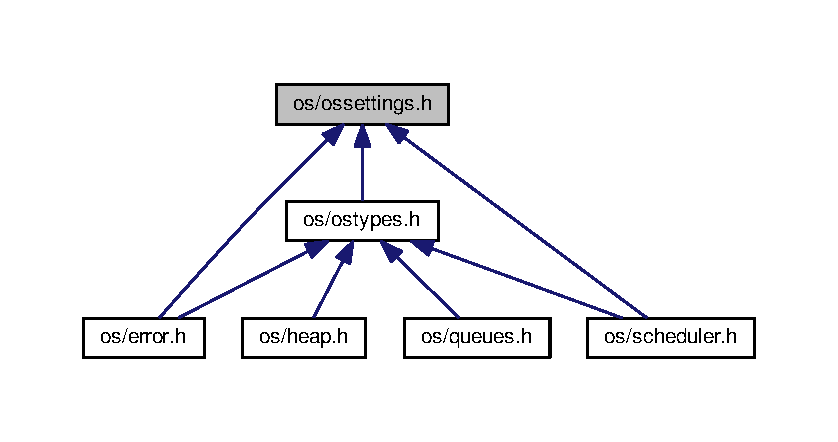
\includegraphics[width=350pt]{ossettings_8h__dep__incl}
\end{center}
\end{figure}
\subsection*{Macros}
\begin{DoxyCompactItemize}
\item 
\mbox{\Hypertarget{ossettings_8h_acb84a306ee37479f97cf0b476560f027}\label{ossettings_8h_acb84a306ee37479f97cf0b476560f027}} 
\#define {\bfseries M\+A\+X\+\_\+\+M\+E\+S\+S\+A\+G\+E\+\_\+\+S\+I\+ZE}~255
\item 
\mbox{\Hypertarget{ossettings_8h_a6d0f30dbf0f5f658209bdfe01e400d40}\label{ossettings_8h_a6d0f30dbf0f5f658209bdfe01e400d40}} 
\#define {\bfseries M\+A\+X\+\_\+\+L\+E\+V\+E\+L\+\_\+\+I\+N\+T\+\_\+\+N\+E\+S\+T\+I\+NG}~3
\item 
\mbox{\Hypertarget{ossettings_8h_aa494389e1ff9b4494ec3f6565b0fcde6}\label{ossettings_8h_aa494389e1ff9b4494ec3f6565b0fcde6}} 
\#define {\bfseries S\+Y\+S\+\_\+\+T\+I\+C\+K\+\_\+\+MS}~100
\item 
\mbox{\Hypertarget{ossettings_8h_a5ed26cf4f2ce5b422c9fd7a00d60ea2b}\label{ossettings_8h_a5ed26cf4f2ce5b422c9fd7a00d60ea2b}} 
\#define {\bfseries S\+Y\+S\+\_\+\+T\+I\+C\+K\+\_\+\+P\+E\+R\+I\+O\+D\+\_\+\+MS}~S\+Y\+S\+\_\+\+T\+I\+C\+K\+\_\+\+MS
\item 
\mbox{\Hypertarget{ossettings_8h_a16ba2eeb8a3b183ecff5652270cf1f4d}\label{ossettings_8h_a16ba2eeb8a3b183ecff5652270cf1f4d}} 
\#define {\bfseries M\+S\+\_\+2\+\_\+\+T\+I\+C\+KS}(MS)~(MS/S\+Y\+S\+\_\+\+T\+I\+C\+K\+\_\+\+MS)
\item 
\mbox{\Hypertarget{ossettings_8h_a63dde392f4d29d54ce7fefc32793be6e}\label{ossettings_8h_a63dde392f4d29d54ce7fefc32793be6e}} 
\#define {\bfseries M\+A\+X\+\_\+\+S\+I\+Z\+E\+\_\+\+T\+A\+S\+K\+\_\+\+N\+A\+ME}~20
\item 
\mbox{\Hypertarget{ossettings_8h_ae429fe1a9a03040b1a337048275f8540}\label{ossettings_8h_ae429fe1a9a03040b1a337048275f8540}} 
\#define {\bfseries M\+A\+X\+\_\+\+N\+U\+M\+B\+E\+R\+\_\+\+O\+F\+\_\+\+T\+A\+S\+KS}~4
\item 
\mbox{\Hypertarget{ossettings_8h_a1b45302695680930829cac31d65e41e1}\label{ossettings_8h_a1b45302695680930829cac31d65e41e1}} 
\#define {\bfseries H\+E\+A\+P\+\_\+\+S\+I\+ZE}~4
\item 
\mbox{\Hypertarget{ossettings_8h_a26d223e387ff89bbbeb5fe1c238f7aa7}\label{ossettings_8h_a26d223e387ff89bbbeb5fe1c238f7aa7}} 
\#define {\bfseries A\+L\+I\+V\+E\+\_\+\+P\+U\+L\+S\+E\+\_\+\+L\+E\+N\+G\+TH}~M\+S\+\_\+2\+\_\+\+T\+I\+C\+KS(200)
\item 
\mbox{\Hypertarget{ossettings_8h_a0e73304dd7fd368f0702df55824d1668}\label{ossettings_8h_a0e73304dd7fd368f0702df55824d1668}} 
\#define {\bfseries C\+O\+N\+V\+E\+R\+T\+\_\+\+N\+E\+W\+L\+I\+NE}
\item 
\mbox{\Hypertarget{ossettings_8h_a0917779e7d7c2d5a3271b5653ad55df9}\label{ossettings_8h_a0917779e7d7c2d5a3271b5653ad55df9}} 
\#define {\bfseries S\+T\+D\+\_\+\+S\+T\+R\+I\+N\+G\+\_\+\+B\+U\+F\+F\+E\+R\+\_\+\+S\+I\+ZE}~128
\item 
\mbox{\Hypertarget{ossettings_8h_ac80a3592e72fd96b772ee47a7d8e0d0a}\label{ossettings_8h_ac80a3592e72fd96b772ee47a7d8e0d0a}} 
\#define {\bfseries D\+E\+B\+U\+G\+\_\+\+M\+O\+DE}~1
\end{DoxyCompactItemize}


\subsection{Detailed Description}
File where all settings take place. 

\begin{DoxyAuthor}{Author}
Maximilian Stiefel 
\end{DoxyAuthor}
\begin{DoxyDate}{Date}
8 Jan 2018 
\end{DoxyDate}

\hypertarget{ostypes_8h}{}\section{os/ostypes.h File Reference}
\label{ostypes_8h}\index{os/ostypes.\+h@{os/ostypes.\+h}}


Different types the operating system uses are defined here.  


{\ttfamily \#include $<$stdint.\+h$>$}\newline
{\ttfamily \#include \char`\"{}ossettings.\+h\char`\"{}}\newline
Include dependency graph for ostypes.\+h\+:\nopagebreak
\begin{figure}[H]
\begin{center}
\leavevmode
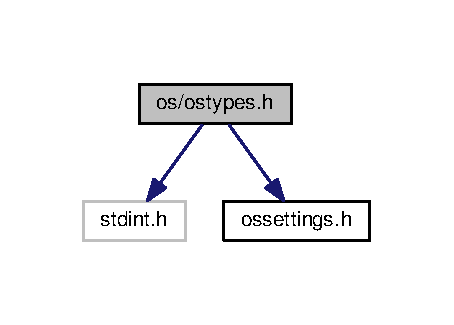
\includegraphics[width=218pt]{ostypes_8h__incl}
\end{center}
\end{figure}
This graph shows which files directly or indirectly include this file\+:
\nopagebreak
\begin{figure}[H]
\begin{center}
\leavevmode
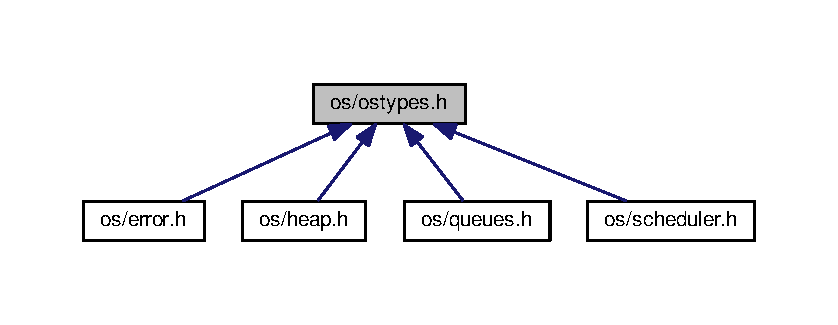
\includegraphics[width=350pt]{ostypes_8h__dep__incl}
\end{center}
\end{figure}
\subsection*{Data Structures}
\begin{DoxyCompactItemize}
\item 
struct \hyperlink{structos_t_c_b__t}{os\+T\+C\+B\+\_\+t}
\item 
struct \hyperlink{structos_q_u_e_u_e__t}{os\+Q\+U\+E\+U\+E\+\_\+t}
\item 
struct \hyperlink{structos_semaphore_handle__t}{os\+Semaphore\+Handle\+\_\+t}
\end{DoxyCompactItemize}
\subsection*{Typedefs}
\begin{DoxyCompactItemize}
\item 
typedef \hyperlink{structos_t_c_b__t}{os\+T\+C\+B\+\_\+t} $\ast$ \hyperlink{ostypes_8h_a7b59ec4a57312624d7d832ba4a8e04be}{os\+Heap\+Node\+\_\+t}
\end{DoxyCompactItemize}
\subsection*{Enumerations}
\begin{DoxyCompactItemize}
\item 
enum \hyperlink{ostypes_8h_ac9a3dac1250976eb655c7a46fceedb8c}{os\+Scheduler\+State\+\_\+t} \{ {\bfseries S\+\_\+\+I\+N\+IT}, 
{\bfseries S\+\_\+\+E\+X\+E\+C\+U\+T\+I\+N\+G\+\_\+\+T\+A\+SK}, 
{\bfseries S\+\_\+\+E\+X\+E\+C\+U\+T\+I\+N\+G\+\_\+\+N\+O\+\_\+\+T\+A\+SK}, 
{\bfseries S\+\_\+\+I\+D\+E\+L\+I\+NG}
 \}
\item 
enum \hyperlink{ostypes_8h_ae410cf8fbf1704d3cedf2e2648b94a55}{os\+Task\+State\+\_\+t} \{ {\bfseries R\+E\+A\+DY}, 
{\bfseries R\+U\+N\+N\+I\+NG}, 
{\bfseries S\+U\+S\+P\+E\+N\+D\+ED}, 
{\bfseries B\+L\+O\+C\+K\+ED}
 \}
\item 
enum \hyperlink{ostypes_8h_acd9f76a1fbd8bc9084ff34add637094f}{os\+Error\+\_\+t} \{ \newline
{\bfseries E\+\_\+\+M\+A\+X\+\_\+\+N\+U\+M\+B\+E\+R\+\_\+\+O\+F\+\_\+\+T\+A\+S\+KS}, 
{\bfseries E\+\_\+\+H\+E\+A\+P\+\_\+\+O\+V\+E\+R\+L\+F\+OW}, 
{\bfseries E\+\_\+\+M\+A\+X\+\_\+\+L\+E\+V\+E\+L\+\_\+\+I\+N\+T\+\_\+\+N\+E\+S\+T\+I\+NG}, 
{\bfseries E\+\_\+\+B\+U\+F\+F\+E\+R\+\_\+\+O\+V\+E\+R\+F\+L\+OW}, 
\newline
{\bfseries E\+\_\+\+N\+U\+L\+L\+\_\+\+F\+O\+R\+B\+I\+D\+D\+EN}, 
{\bfseries E\+\_\+\+W\+R\+O\+N\+G\+\_\+\+U\+S\+A\+G\+E\+\_\+\+O\+F\+\_\+\+P\+R\+I\+N\+TF}, 
{\bfseries E\+\_\+\+U\+S\+A\+R\+T\+\_\+\+R\+X\+\_\+\+B\+U\+F\+F\+E\+R\+\_\+\+O\+V\+E\+R\+L\+OW}, 
{\bfseries E\+\_\+\+U\+S\+A\+R\+T\+\_\+\+T\+X\+\_\+\+B\+U\+F\+F\+E\+R\+\_\+\+O\+V\+E\+R\+L\+OW}, 
\newline
{\bfseries E\+\_\+\+P\+R\+I\+N\+T\+F\+\_\+\+W\+E\+N\+T\+\_\+\+W\+R\+O\+NG}
 \}
\item 
enum \hyperlink{ostypes_8h_a5c976ef3f21f800d03382e5cc640c362}{os\+Warning\+\_\+t} \{ {\bfseries W\+\_\+\+S\+Y\+S\+\_\+\+T\+I\+M\+E\+R\+\_\+\+O\+V\+E\+R\+F\+L\+OW}
 \}
\item 
\mbox{\Hypertarget{ostypes_8h_ad68cf10efc310f9689628bde190fe714}\label{ostypes_8h_ad68cf10efc310f9689628bde190fe714}} 
enum {\bfseries os\+Semaphore\+Binary\+\_\+t} \{ {\bfseries A\+V\+A\+I\+L\+A\+B\+LE}, 
{\bfseries T\+A\+K\+EN}
 \}
\item 
\mbox{\Hypertarget{ostypes_8h_ab218649e29adcb54aefa674dc6f17acf}\label{ostypes_8h_ab218649e29adcb54aefa674dc6f17acf}} 
enum {\bfseries os\+Semaphore\+Type\+\_\+t} \{ {\bfseries B\+I\+N\+A\+RY}
 \}
\end{DoxyCompactItemize}


\subsection{Detailed Description}
Different types the operating system uses are defined here. 

\begin{DoxyAuthor}{Author}
Maximilian Stiefel 
\end{DoxyAuthor}
\begin{DoxyDate}{Date}
8 Jan 2018 
\end{DoxyDate}


\subsection{Typedef Documentation}
\mbox{\Hypertarget{ostypes_8h_a7b59ec4a57312624d7d832ba4a8e04be}\label{ostypes_8h_a7b59ec4a57312624d7d832ba4a8e04be}} 
\index{ostypes.\+h@{ostypes.\+h}!os\+Heap\+Node\+\_\+t@{os\+Heap\+Node\+\_\+t}}
\index{os\+Heap\+Node\+\_\+t@{os\+Heap\+Node\+\_\+t}!ostypes.\+h@{ostypes.\+h}}
\subsubsection{\texorpdfstring{os\+Heap\+Node\+\_\+t}{osHeapNode\_t}}
{\footnotesize\ttfamily typedef \hyperlink{structos_t_c_b__t}{os\+T\+C\+B\+\_\+t}$\ast$ \hyperlink{ostypes_8h_a7b59ec4a57312624d7d832ba4a8e04be}{os\+Heap\+Node\+\_\+t}}

Data type to hold a pointer to a T\+CB. 

\subsection{Enumeration Type Documentation}
\mbox{\Hypertarget{ostypes_8h_acd9f76a1fbd8bc9084ff34add637094f}\label{ostypes_8h_acd9f76a1fbd8bc9084ff34add637094f}} 
\index{ostypes.\+h@{ostypes.\+h}!os\+Error\+\_\+t@{os\+Error\+\_\+t}}
\index{os\+Error\+\_\+t@{os\+Error\+\_\+t}!ostypes.\+h@{ostypes.\+h}}
\subsubsection{\texorpdfstring{os\+Error\+\_\+t}{osError\_t}}
{\footnotesize\ttfamily enum \hyperlink{ostypes_8h_acd9f76a1fbd8bc9084ff34add637094f}{os\+Error\+\_\+t}}

Enum to hold all possible error codes. \mbox{\Hypertarget{ostypes_8h_ac9a3dac1250976eb655c7a46fceedb8c}\label{ostypes_8h_ac9a3dac1250976eb655c7a46fceedb8c}} 
\index{ostypes.\+h@{ostypes.\+h}!os\+Scheduler\+State\+\_\+t@{os\+Scheduler\+State\+\_\+t}}
\index{os\+Scheduler\+State\+\_\+t@{os\+Scheduler\+State\+\_\+t}!ostypes.\+h@{ostypes.\+h}}
\subsubsection{\texorpdfstring{os\+Scheduler\+State\+\_\+t}{osSchedulerState\_t}}
{\footnotesize\ttfamily enum \hyperlink{ostypes_8h_ac9a3dac1250976eb655c7a46fceedb8c}{os\+Scheduler\+State\+\_\+t}}

Enum for scheduler state. \mbox{\Hypertarget{ostypes_8h_ae410cf8fbf1704d3cedf2e2648b94a55}\label{ostypes_8h_ae410cf8fbf1704d3cedf2e2648b94a55}} 
\index{ostypes.\+h@{ostypes.\+h}!os\+Task\+State\+\_\+t@{os\+Task\+State\+\_\+t}}
\index{os\+Task\+State\+\_\+t@{os\+Task\+State\+\_\+t}!ostypes.\+h@{ostypes.\+h}}
\subsubsection{\texorpdfstring{os\+Task\+State\+\_\+t}{osTaskState\_t}}
{\footnotesize\ttfamily enum \hyperlink{ostypes_8h_ae410cf8fbf1704d3cedf2e2648b94a55}{os\+Task\+State\+\_\+t}}

Enum for task states. \mbox{\Hypertarget{ostypes_8h_a5c976ef3f21f800d03382e5cc640c362}\label{ostypes_8h_a5c976ef3f21f800d03382e5cc640c362}} 
\index{ostypes.\+h@{ostypes.\+h}!os\+Warning\+\_\+t@{os\+Warning\+\_\+t}}
\index{os\+Warning\+\_\+t@{os\+Warning\+\_\+t}!ostypes.\+h@{ostypes.\+h}}
\subsubsection{\texorpdfstring{os\+Warning\+\_\+t}{osWarning\_t}}
{\footnotesize\ttfamily enum \hyperlink{ostypes_8h_a5c976ef3f21f800d03382e5cc640c362}{os\+Warning\+\_\+t}}

Enum to hold all possible warning codes. 
\hypertarget{printf_8h}{}\section{os/printf.h File Reference}
\label{printf_8h}\index{os/printf.\+h@{os/printf.\+h}}


Lightweight version of G\+NU printf.  


{\ttfamily \#include $<$stdio.\+h$>$}\newline
{\ttfamily \#include $<$stdarg.\+h$>$}\newline
{\ttfamily \#include \char`\"{}stm32f10x.\+h\char`\"{}}\newline
Include dependency graph for printf.\+h\+:\nopagebreak
\begin{figure}[H]
\begin{center}
\leavevmode
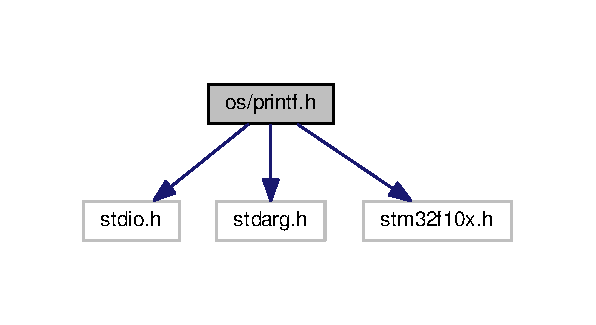
\includegraphics[width=286pt]{printf_8h__incl}
\end{center}
\end{figure}
\subsection*{Functions}
\begin{DoxyCompactItemize}
\item 
int \hyperlink{printf_8h_ae2b707b3f94f0857c447e83c833b068a}{os\+Printf} (const char $\ast$iformat,...)
\end{DoxyCompactItemize}


\subsection{Detailed Description}
Lightweight version of G\+NU printf. 

\begin{DoxyAuthor}{Author}
Maximilian Stiefel 
\end{DoxyAuthor}
\begin{DoxyDate}{Date}
8 Jan 2018 
\end{DoxyDate}


\subsection{Function Documentation}
\mbox{\Hypertarget{printf_8h_ae2b707b3f94f0857c447e83c833b068a}\label{printf_8h_ae2b707b3f94f0857c447e83c833b068a}} 
\index{printf.\+h@{printf.\+h}!os\+Printf@{os\+Printf}}
\index{os\+Printf@{os\+Printf}!printf.\+h@{printf.\+h}}
\subsubsection{\texorpdfstring{os\+Printf()}{osPrintf()}}
{\footnotesize\ttfamily int os\+Printf (\begin{DoxyParamCaption}\item[{const char $\ast$}]{iformat,  }\item[{}]{... }\end{DoxyParamCaption})}

printf to be used by the OS user. Can be ported to another platform easily by just using another function to transmit one string with the U\+S\+A\+RT.


\begin{DoxyParams}{Parameters}
{\em iformat} & Currently supported are d integers c single characters s C strings f Floats with 4 decimals \%.xf Floats with x decimals \\
\hline
\end{DoxyParams}

\begin{DoxyRetVals}{Return values}
{\em Returns} & the number of characters printed (S\+U\+C\+C\+E\+SS) or -\/1 (F\+A\+I\+L\+U\+RE). \\
\hline
\end{DoxyRetVals}

\hypertarget{queues_8h}{}\section{os/queues.h File Reference}
\label{queues_8h}\index{os/queues.\+h@{os/queues.\+h}}


Implementation for queues.  


{\ttfamily \#include $<$stm32f10x.\+h$>$}\newline
{\ttfamily \#include \char`\"{}ostypes.\+h\char`\"{}}\newline
{\ttfamily \#include $<$stdlib.\+h$>$}\newline
Include dependency graph for queues.\+h\+:\nopagebreak
\begin{figure}[H]
\begin{center}
\leavevmode
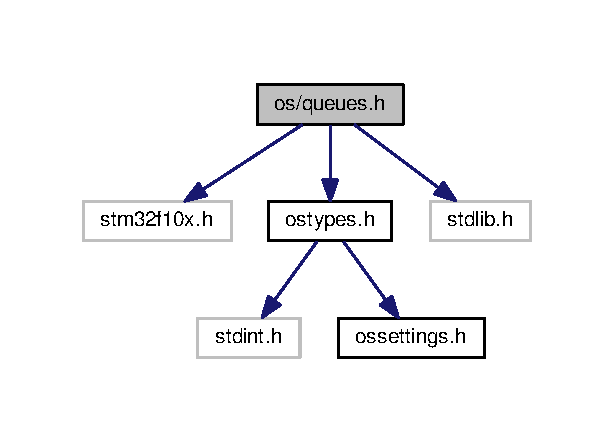
\includegraphics[width=295pt]{queues_8h__incl}
\end{center}
\end{figure}
\subsection*{Functions}
\begin{DoxyCompactItemize}
\item 
void \hyperlink{queues_8h_a164dd36f8a083fd39b238b6d05910320}{os\+Q\+Init} (\hyperlink{structos_q_u_e_u_e__t}{os\+Q\+U\+E\+U\+E\+\_\+t} $\ast$q, size\+\_\+t ivarsize, uint16\+\_\+t iqsize, void $\ast$istart)
\item 
uint8\+\_\+t \hyperlink{queues_8h_a78b4d06b91514e747007d1cc03029b44}{os\+Enqueue} (\hyperlink{structos_q_u_e_u_e__t}{os\+Q\+U\+E\+U\+E\+\_\+t} $\ast$q, void $\ast$data)
\item 
uint8\+\_\+t \hyperlink{queues_8h_a0037677933e9d9d089327009032edf2c}{os\+Dequeue} (\hyperlink{structos_q_u_e_u_e__t}{os\+Q\+U\+E\+U\+E\+\_\+t} $\ast$q, void $\ast$data)
\end{DoxyCompactItemize}


\subsection{Detailed Description}
Implementation for queues. 

\begin{DoxyAuthor}{Author}
Maximilian Stiefel 
\end{DoxyAuthor}
\begin{DoxyDate}{Date}
8 Jan 2018 
\end{DoxyDate}


\subsection{Function Documentation}
\mbox{\Hypertarget{queues_8h_a0037677933e9d9d089327009032edf2c}\label{queues_8h_a0037677933e9d9d089327009032edf2c}} 
\index{queues.\+h@{queues.\+h}!os\+Dequeue@{os\+Dequeue}}
\index{os\+Dequeue@{os\+Dequeue}!queues.\+h@{queues.\+h}}
\subsubsection{\texorpdfstring{os\+Dequeue()}{osDequeue()}}
{\footnotesize\ttfamily uint8\+\_\+t os\+Dequeue (\begin{DoxyParamCaption}\item[{\hyperlink{structos_q_u_e_u_e__t}{os\+Q\+U\+E\+U\+E\+\_\+t} $\ast$}]{q,  }\item[{void $\ast$}]{data }\end{DoxyParamCaption})}

Copy data from the q.


\begin{DoxyParams}{Parameters}
{\em q} & Q we are talking about. \\
\hline
{\em data} & Pointer to a local variable where the data from the q shall end up. \\
\hline
\end{DoxyParams}

\begin{DoxyRetVals}{Return values}
{\em 1} & (data successfully copied) or 0 (q is empty). \\
\hline
\end{DoxyRetVals}
\mbox{\Hypertarget{queues_8h_a78b4d06b91514e747007d1cc03029b44}\label{queues_8h_a78b4d06b91514e747007d1cc03029b44}} 
\index{queues.\+h@{queues.\+h}!os\+Enqueue@{os\+Enqueue}}
\index{os\+Enqueue@{os\+Enqueue}!queues.\+h@{queues.\+h}}
\subsubsection{\texorpdfstring{os\+Enqueue()}{osEnqueue()}}
{\footnotesize\ttfamily uint8\+\_\+t os\+Enqueue (\begin{DoxyParamCaption}\item[{\hyperlink{structos_q_u_e_u_e__t}{os\+Q\+U\+E\+U\+E\+\_\+t} $\ast$}]{q,  }\item[{void $\ast$}]{data }\end{DoxyParamCaption})}

Copy data to the q.


\begin{DoxyParams}{Parameters}
{\em q} & Q we are talking about. \\
\hline
{\em data} & Pointer to a local variable where data is stored. \\
\hline
\end{DoxyParams}

\begin{DoxyRetVals}{Return values}
{\em 1} & (data successfully copied) or 0 (q is full). \\
\hline
\end{DoxyRetVals}
\mbox{\Hypertarget{queues_8h_a164dd36f8a083fd39b238b6d05910320}\label{queues_8h_a164dd36f8a083fd39b238b6d05910320}} 
\index{queues.\+h@{queues.\+h}!os\+Q\+Init@{os\+Q\+Init}}
\index{os\+Q\+Init@{os\+Q\+Init}!queues.\+h@{queues.\+h}}
\subsubsection{\texorpdfstring{os\+Q\+Init()}{osQInit()}}
{\footnotesize\ttfamily void os\+Q\+Init (\begin{DoxyParamCaption}\item[{\hyperlink{structos_q_u_e_u_e__t}{os\+Q\+U\+E\+U\+E\+\_\+t} $\ast$}]{q,  }\item[{size\+\_\+t}]{ivarsize,  }\item[{uint16\+\_\+t}]{iqsize,  }\item[{void $\ast$}]{istart }\end{DoxyParamCaption})}

Function to initialize a queue properly.


\begin{DoxyParams}{Parameters}
{\em q} & Pointer to the memory where the q is stored. \\
\hline
{\em ivarsize} & Size of the variable type stored in the q in bytes. \\
\hline
{\em iqsize} & Number of slots of the q. \\
\hline
{\em istart} & Pointer to the array where the actual data of the q is stored. \\
\hline
\end{DoxyParams}

\hypertarget{scheduler_8h}{}\section{os/scheduler.h File Reference}
\label{scheduler_8h}\index{os/scheduler.\+h@{os/scheduler.\+h}}


Scheduler of the operating system.  


{\ttfamily \#include $<$stdlib.\+h$>$}\newline
{\ttfamily \#include $<$stdint.\+h$>$}\newline
{\ttfamily \#include \char`\"{}ossettings.\+h\char`\"{}}\newline
{\ttfamily \#include \char`\"{}ostypes.\+h\char`\"{}}\newline
Include dependency graph for scheduler.\+h\+:\nopagebreak
\begin{figure}[H]
\begin{center}
\leavevmode
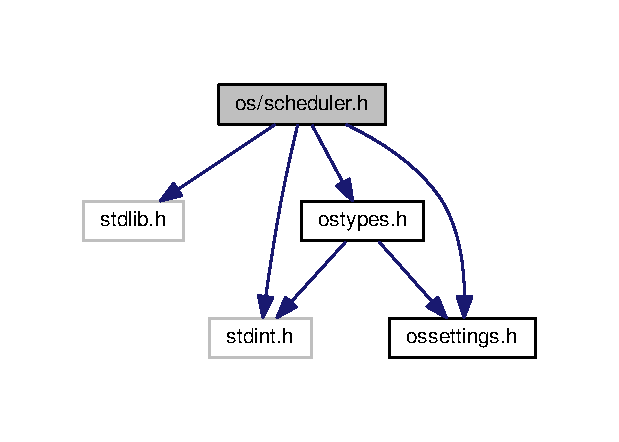
\includegraphics[width=297pt]{scheduler_8h__incl}
\end{center}
\end{figure}
\subsection*{Functions}
\begin{DoxyCompactItemize}
\item 
uint32\+\_\+t \hyperlink{scheduler_8h_ac59673f226b3291f835a0faf010ad409}{os\+Scheduler\+Get\+SysT} (void)
\item 
uint8\+\_\+t \hyperlink{scheduler_8h_a76739fd1872ff1f867ea41e853131a21}{os\+Task\+Create} (void($\ast$ifnc\+\_\+ptr)(void $\ast$), char $\ast$itask\+\_\+name, void $\ast$iarguments, uint8\+\_\+t ipriority, const \hyperlink{structos_t_c_b__t}{os\+T\+C\+B\+\_\+t} $\ast$o\+Task\+Handle)
\item 
void \hyperlink{scheduler_8h_a790ca9c0d2362305790eb3c4002e3da9}{os\+Task\+Delete} (\hyperlink{structos_t_c_b__t}{os\+T\+C\+B\+\_\+t} $\ast$iotask)
\item 
void \hyperlink{scheduler_8h_ae1e7565174265c0107749d7cdf486c01}{os\+Task\+Delay} (uint8\+\_\+t idelay)
\item 
void \hyperlink{scheduler_8h_ae4c7af5e41838a9299b00d455fb8f454}{os\+Task\+Delay\+Until} (uint32\+\_\+t iwakeup\+\_\+time, uint8\+\_\+t idelay)
\item 
void \hyperlink{scheduler_8h_ada28e10d8b44223004cab16b201df2d7}{os\+Run\+Scheduler} (void)
\item 
void \hyperlink{scheduler_8h_acd27cd0dcb4e193125968decdd238ff9}{os\+Print\+Task} (uint8\+\_\+t iindex)
\item 
void \hyperlink{scheduler_8h_ad4967a4ccbd9e8901a1d79a9ee3ca79b}{os\+Print\+All\+Tasks} (void)
\end{DoxyCompactItemize}


\subsection{Detailed Description}
Scheduler of the operating system. 

\begin{DoxyAuthor}{Author}
Maximilian Stiefel 
\end{DoxyAuthor}
\begin{DoxyDate}{Date}
8 Jan 2018 
\end{DoxyDate}


\subsection{Function Documentation}
\mbox{\Hypertarget{scheduler_8h_ad4967a4ccbd9e8901a1d79a9ee3ca79b}\label{scheduler_8h_ad4967a4ccbd9e8901a1d79a9ee3ca79b}} 
\index{scheduler.\+h@{scheduler.\+h}!os\+Print\+All\+Tasks@{os\+Print\+All\+Tasks}}
\index{os\+Print\+All\+Tasks@{os\+Print\+All\+Tasks}!scheduler.\+h@{scheduler.\+h}}
\subsubsection{\texorpdfstring{os\+Print\+All\+Tasks()}{osPrintAllTasks()}}
{\footnotesize\ttfamily void os\+Print\+All\+Tasks (\begin{DoxyParamCaption}\item[{void}]{ }\end{DoxyParamCaption})}

Print all information about all tasks. \mbox{\Hypertarget{scheduler_8h_acd27cd0dcb4e193125968decdd238ff9}\label{scheduler_8h_acd27cd0dcb4e193125968decdd238ff9}} 
\index{scheduler.\+h@{scheduler.\+h}!os\+Print\+Task@{os\+Print\+Task}}
\index{os\+Print\+Task@{os\+Print\+Task}!scheduler.\+h@{scheduler.\+h}}
\subsubsection{\texorpdfstring{os\+Print\+Task()}{osPrintTask()}}
{\footnotesize\ttfamily void os\+Print\+Task (\begin{DoxyParamCaption}\item[{uint8\+\_\+t}]{iindex }\end{DoxyParamCaption})}

Print all information about one task.


\begin{DoxyParams}{Parameters}
{\em iindex} & Index in the T\+CB array. \\
\hline
\end{DoxyParams}
\mbox{\Hypertarget{scheduler_8h_ada28e10d8b44223004cab16b201df2d7}\label{scheduler_8h_ada28e10d8b44223004cab16b201df2d7}} 
\index{scheduler.\+h@{scheduler.\+h}!os\+Run\+Scheduler@{os\+Run\+Scheduler}}
\index{os\+Run\+Scheduler@{os\+Run\+Scheduler}!scheduler.\+h@{scheduler.\+h}}
\subsubsection{\texorpdfstring{os\+Run\+Scheduler()}{osRunScheduler()}}
{\footnotesize\ttfamily void os\+Run\+Scheduler (\begin{DoxyParamCaption}\item[{void}]{ }\end{DoxyParamCaption})}

System core. Scheduler needs to be executed by a timer interrupt. \mbox{\Hypertarget{scheduler_8h_ac59673f226b3291f835a0faf010ad409}\label{scheduler_8h_ac59673f226b3291f835a0faf010ad409}} 
\index{scheduler.\+h@{scheduler.\+h}!os\+Scheduler\+Get\+SysT@{os\+Scheduler\+Get\+SysT}}
\index{os\+Scheduler\+Get\+SysT@{os\+Scheduler\+Get\+SysT}!scheduler.\+h@{scheduler.\+h}}
\subsubsection{\texorpdfstring{os\+Scheduler\+Get\+Sys\+T()}{osSchedulerGetSysT()}}
{\footnotesize\ttfamily uint32\+\_\+t os\+Scheduler\+Get\+SysT (\begin{DoxyParamCaption}\item[{void}]{ }\end{DoxyParamCaption})}

Get the system time.


\begin{DoxyRetVals}{Return values}
{\em Gives} & back the number of ticks since system has been initialized. \\
\hline
\end{DoxyRetVals}
\mbox{\Hypertarget{scheduler_8h_a76739fd1872ff1f867ea41e853131a21}\label{scheduler_8h_a76739fd1872ff1f867ea41e853131a21}} 
\index{scheduler.\+h@{scheduler.\+h}!os\+Task\+Create@{os\+Task\+Create}}
\index{os\+Task\+Create@{os\+Task\+Create}!scheduler.\+h@{scheduler.\+h}}
\subsubsection{\texorpdfstring{os\+Task\+Create()}{osTaskCreate()}}
{\footnotesize\ttfamily uint8\+\_\+t os\+Task\+Create (\begin{DoxyParamCaption}\item[{void($\ast$)(void $\ast$)}]{ifnc\+\_\+ptr,  }\item[{char $\ast$}]{itask\+\_\+name,  }\item[{void $\ast$}]{iarguments,  }\item[{uint8\+\_\+t}]{ipriority,  }\item[{const \hyperlink{structos_t_c_b__t}{os\+T\+C\+B\+\_\+t} $\ast$}]{o\+Task\+Handle }\end{DoxyParamCaption})}

Spawn a task.


\begin{DoxyParams}{Parameters}
{\em ifnc\+\_\+ptr} & Pointer to the task function. \\
\hline
{\em itask\+\_\+name} & Internal task name. \\
\hline
{\em iarguments} & Enables passing user-\/defined arguments to the task. \\
\hline
{\em ipriority} & A higher value means a higher priority of the task. \\
\hline
{\em o\+Task\+Handle} & Pointer to T\+CB. \\
\hline
\end{DoxyParams}

\begin{DoxyRetVals}{Return values}
{\em 1} & (task has been spawned) or 0 (F\+A\+I\+L\+ED) \\
\hline
\end{DoxyRetVals}
\mbox{\Hypertarget{scheduler_8h_ae1e7565174265c0107749d7cdf486c01}\label{scheduler_8h_ae1e7565174265c0107749d7cdf486c01}} 
\index{scheduler.\+h@{scheduler.\+h}!os\+Task\+Delay@{os\+Task\+Delay}}
\index{os\+Task\+Delay@{os\+Task\+Delay}!scheduler.\+h@{scheduler.\+h}}
\subsubsection{\texorpdfstring{os\+Task\+Delay()}{osTaskDelay()}}
{\footnotesize\ttfamily void os\+Task\+Delay (\begin{DoxyParamCaption}\item[{uint8\+\_\+t}]{idelay }\end{DoxyParamCaption})}

Delay function. DO N\+OT U\+SE F\+OR P\+E\+R\+I\+O\+D\+IC T\+A\+S\+K\+S!


\begin{DoxyParams}{Parameters}
{\em idelay} & Delay in system ticks. \\
\hline
\end{DoxyParams}
\mbox{\Hypertarget{scheduler_8h_ae4c7af5e41838a9299b00d455fb8f454}\label{scheduler_8h_ae4c7af5e41838a9299b00d455fb8f454}} 
\index{scheduler.\+h@{scheduler.\+h}!os\+Task\+Delay\+Until@{os\+Task\+Delay\+Until}}
\index{os\+Task\+Delay\+Until@{os\+Task\+Delay\+Until}!scheduler.\+h@{scheduler.\+h}}
\subsubsection{\texorpdfstring{os\+Task\+Delay\+Until()}{osTaskDelayUntil()}}
{\footnotesize\ttfamily void os\+Task\+Delay\+Until (\begin{DoxyParamCaption}\item[{uint32\+\_\+t}]{iwakeup\+\_\+time,  }\item[{uint8\+\_\+t}]{idelay }\end{DoxyParamCaption})}

Delay until function. DO U\+SE F\+OR P\+E\+R\+I\+O\+D\+IC T\+A\+S\+K\+S!


\begin{DoxyParams}{Parameters}
{\em iwakeup\+\_\+time} & Time when the task execution started. \\
\hline
{\em idelay} & Number of system ticks until the task shall be executed again. \\
\hline
\end{DoxyParams}
\mbox{\Hypertarget{scheduler_8h_a790ca9c0d2362305790eb3c4002e3da9}\label{scheduler_8h_a790ca9c0d2362305790eb3c4002e3da9}} 
\index{scheduler.\+h@{scheduler.\+h}!os\+Task\+Delete@{os\+Task\+Delete}}
\index{os\+Task\+Delete@{os\+Task\+Delete}!scheduler.\+h@{scheduler.\+h}}
\subsubsection{\texorpdfstring{os\+Task\+Delete()}{osTaskDelete()}}
{\footnotesize\ttfamily void os\+Task\+Delete (\begin{DoxyParamCaption}\item[{\hyperlink{structos_t_c_b__t}{os\+T\+C\+B\+\_\+t} $\ast$}]{iotask }\end{DoxyParamCaption})}

Simply delete task by setting the function pointer to N\+U\+LL.


\begin{DoxyParams}{Parameters}
{\em iotask} & Pointer to T\+CB. \\
\hline
\end{DoxyParams}

\hypertarget{semaphore_8h}{}\section{os/semaphore.h File Reference}
\label{semaphore_8h}\index{os/semaphore.\+h@{os/semaphore.\+h}}


Mechanisms to prevent race conditions for the operating system.  




\subsection{Detailed Description}
Mechanisms to prevent race conditions for the operating system. 

\begin{DoxyAuthor}{Author}
Maximilian Stiefel 
\end{DoxyAuthor}
\begin{DoxyDate}{Date}
8 Jan 2018 
\end{DoxyDate}

%--- End generated contents ---

% Index
\backmatter
\newpage
\phantomsection
\clearemptydoublepage
\addcontentsline{toc}{chapter}{Index}
\printindex

\end{document}
